\documentclass[11pt,a4paper]{article}

\usepackage[T1]{fontenc}
\usepackage[utf8]{inputenc}
\usepackage{lmodern}
\usepackage[scaled=0.92]{helvet}
\renewcommand{\familydefault}{\sfdefault}
\usepackage[margin=2.2cm,top=2.4cm,bottom=2.4cm]{geometry}
\usepackage{microtype}
\usepackage{graphicx}
\usepackage{xcolor}
\usepackage{tabularx}
\usepackage{booktabs}
\usepackage{enumitem}
\usepackage{titlesec}
\usepackage{fancyhdr}
\usepackage{listings}
\usepackage[most]{tcolorbox}
\usepackage{tikz}
\usetikzlibrary{positioning,arrows.meta}
\usepackage[hidelinks]{hyperref}

% ---------- colours ----------
\definecolor{navy}{HTML}{14213D}
\definecolor{amber}{HTML}{FCA311}
\definecolor{teal}{HTML}{2A9D8F}
\definecolor{coral}{HTML}{E76F51}
\definecolor{slate}{HTML}{5C6B80}
\definecolor{tint}{HTML}{EEF2F7}
\definecolor{codebg}{HTML}{1E2A3A}
\definecolor{winblue}{HTML}{0067B8}
\definecolor{ubuorange}{HTML}{C2410C}
\definecolor{checkgreen}{HTML}{2E7D32}

\hypersetup{colorlinks=true,linkcolor=navy,urlcolor=teal}
\setlength{\parindent}{0pt}
\setlength{\parskip}{0.5em}
\setlist{itemsep=0.2em,topsep=0.3em}

% ---------- headings ----------
\titleformat{\section}{\Large\bfseries\color{navy}}{\colorbox{amber}{\makebox[1.5em]{\color{navy}\thesection}}}{0.6em}{}
\titleformat{\subsection}{\large\bfseries\color{navy}}{\thesubsection}{0.6em}{}
\titlespacing*{\section}{0pt}{1.4em}{0.6em}
\titlespacing*{\subsection}{0pt}{1.1em}{0.4em}
\renewcommand{\thesection}{\Alph{section}}

% ---------- header and footer ----------
\pagestyle{fancy}
\fancyhf{}
\fancyhead[L]{\small\color{slate}VS Code, the UT HPC cluster, and a Vision Transformer}
\fancyhead[R]{\small\color{slate}GenAI Models and Robotic Applications}
\fancyfoot[L]{\small\color{slate}\url{https://github.com/alicamdal/vscode-hpc-tutorial}}
\fancyfoot[R]{\small\color{slate}\thepage}
\renewcommand{\headrulewidth}{0pt}

% ---------- code ----------
\lstdefinestyle{term}{
  basicstyle=\ttfamily\small\color{white},
  columns=fullflexible, keepspaces=true, breaklines=true,
  breakatwhitespace=false, showstringspaces=false,
  upquote=true, literate={~}{{\textasciitilde}}1,
}
\newtcblisting{cmd}[1][]{
  listing only, colback=codebg, colframe=codebg, arc=1.5mm,
  boxrule=0pt, left=3mm, right=3mm, top=1.5mm, bottom=1.5mm,
  listing options={style=term}, #1}
\newtcblisting{wincmd}{
  listing only, colback=codebg, colframe=winblue, arc=1.5mm, boxrule=0.6pt,
  left=3mm, right=3mm, top=1.5mm, bottom=1.5mm, listing options={style=term},
  title={\small\bfseries Windows (PowerShell)}, coltitle=white, colbacktitle=winblue,
  attach boxed title to top left={yshift=-2mm,xshift=3mm}, boxed title style={arc=1mm,boxrule=0pt},
  enhanced, top=3mm}
\newtcblisting{ubucmd}{
  listing only, colback=codebg, colframe=ubuorange, arc=1.5mm, boxrule=0.6pt,
  left=3mm, right=3mm, top=1.5mm, bottom=1.5mm, listing options={style=term},
  title={\small\bfseries Ubuntu}, coltitle=white, colbacktitle=ubuorange,
  attach boxed title to top left={yshift=-2mm,xshift=3mm}, boxed title style={arc=1mm,boxrule=0pt},
  enhanced, top=3mm}
\newtcblisting{outbox}{
  listing only, colback=tint, colframe=tint, arc=1.5mm, boxrule=0pt,
  left=3mm, right=3mm, top=1.5mm, bottom=1.5mm,
  listing options={basicstyle=\ttfamily\footnotesize\color{navy},columns=fullflexible,keepspaces=true,breaklines=true}}

% ---------- callouts ----------
\newtcolorbox{checkbox}{enhanced, colback=checkgreen!6, colframe=checkgreen, boxrule=0pt,
  leftrule=0pt, arc=1.5mm, left=3mm, right=3mm, top=1.5mm, bottom=1.5mm,
  fontupper=\small\raggedright, before upper={\textbf{\color{checkgreen}Check:\ }}}
\newtcolorbox{notebox}[1][Note]{enhanced, colback=amber!10, colframe=amber!10, arc=1.5mm,
  left=3mm, right=3mm, top=1.5mm, bottom=1.5mm, fontupper=\small\raggedright,
  before upper={\textbf{\color{navy}#1:\ }}}
\newcommand{\win}{\textbf{\color{winblue}Windows:}\ }
\newcommand{\ubu}{\textbf{\color{ubuorange}Ubuntu:}\ }
\newcommand{\key}[1]{\tcbox[on line, colback=tint, colframe=slate!60, boxrule=0.4pt, arc=0.8mm,
  left=0.8mm, right=0.8mm, top=0.2mm, bottom=0.2mm]{\small\ttfamily #1}}
\newcommand{\menu}[1]{\textsf{\textbf{#1}}}
\newcommand{\code}[1]{\colorbox{tint}{\ttfamily\small #1}}

% Screenshot: shows the image when it exists, a placeholder box otherwise.
\newcommand{\shot}[3][0.85]{%
  \begin{center}
  \IfFileExists{img/#2}{%
    \includegraphics[width=#1\linewidth]{img/#2}%
  }{%
    \fcolorbox{slate}{tint}{\parbox[c][3.5cm][c]{#1\linewidth}{\centering\small\color{slate}Screenshot: #3}}%
  }\\[0.3em]
  {\small\color{slate}#3}
  \end{center}}

\begin{document}

% ================= cover =================
\thispagestyle{empty}
\begin{tikzpicture}[remember picture,overlay]
  \fill[navy] (current page.north west) rectangle ([yshift=-11cm]current page.north east);
\end{tikzpicture}
\vspace*{0.6cm}
{\color{amber}\large\bfseries GenAI Models and Robotic Applications (2026-1B) \quad|\quad Tutorial}\par
\vspace{0.8cm}
{\color{white}\fontsize{30}{36}\selectfont\bfseries From your laptop\\[0.15em] to a GPU cluster\par}
\vspace{0.5cm}
{\color{white}\Large VS Code, the UT HPC cluster, and a look inside a Vision Transformer\par}
\vspace{0.6cm}
{\color{amber}\large Step-by-step guide for Windows and Ubuntu\par}
\vspace{2.2cm}

\begin{minipage}[t]{0.55\linewidth}
\textbf{\color{navy}What you will do}
\begin{enumerate}[leftmargin=1.4em]
  \item Install VS Code, Git, Python, and eduVPN.
  \item Connect VS Code to the UT HPC cluster.
  \item Run a small GPU job on the cluster.
  \item Run a Vision Transformer on your laptop and see how it reads an image.
  \item (Optional) Add an AI coding assistant.
\end{enumerate}
\vspace{0.4em}
\textbf{\color{navy}Code and this guide}\\
\url{https://github.com/alicamdal/vscode-hpc-tutorial}

\vspace{0.6em}
\textbf{\color{navy}Tutorial}\\
20 November 2026 \quad|\quad Ali Camdal, PhD candidate, ITC, University of Twente
\end{minipage}\hfill
\begin{minipage}[t]{0.38\linewidth}\vspace{0pt}
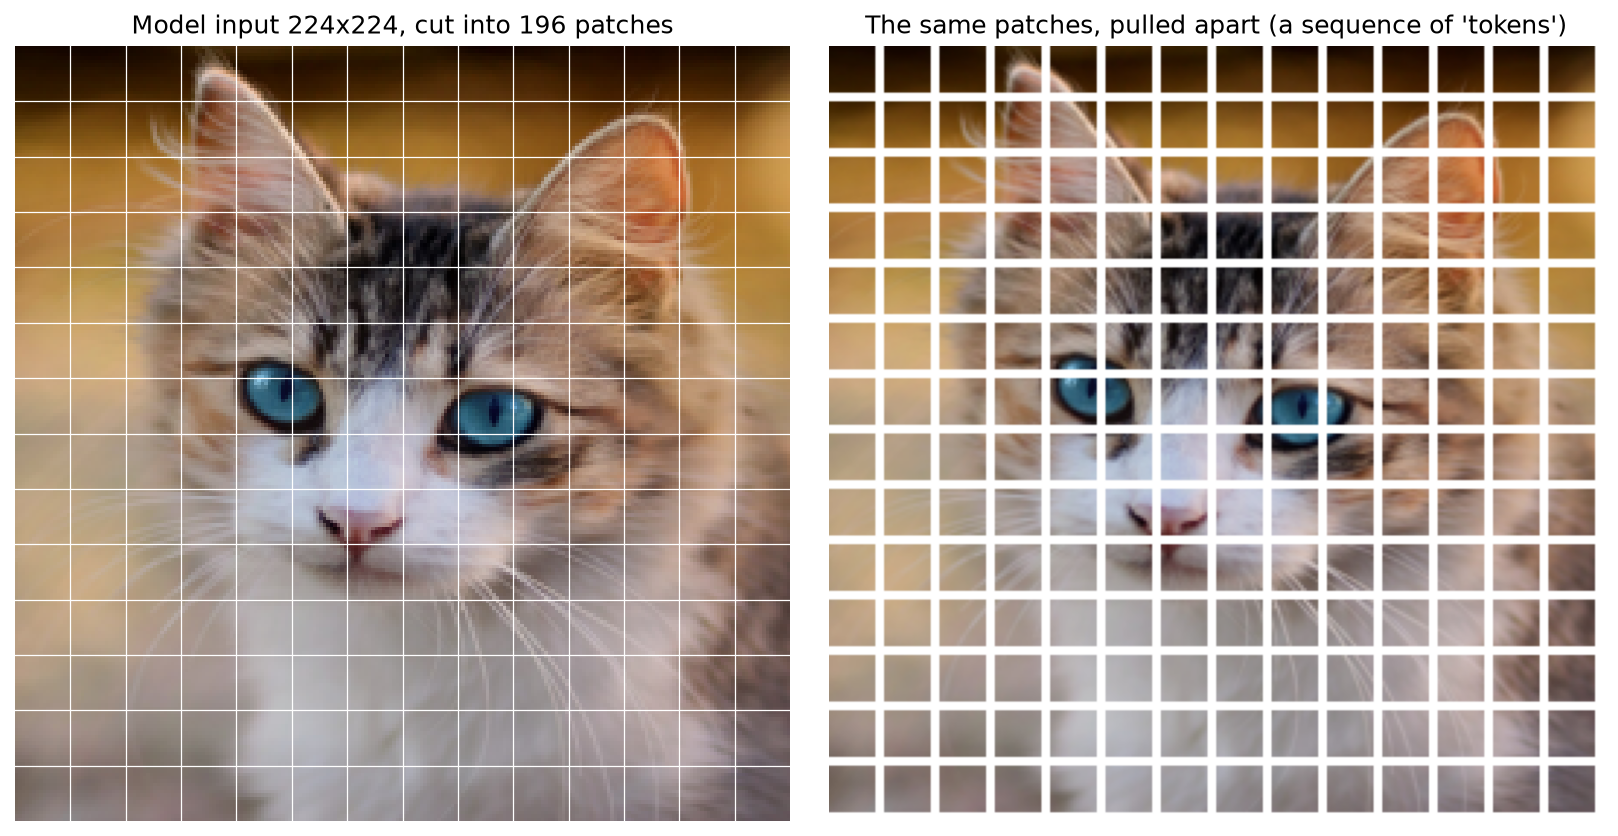
\includegraphics[width=\linewidth]{img/demo_1_patches.png}\\[-0.2em]
{\small\color{slate}A Vision Transformer cuts an image into patches.}
\end{minipage}

\newpage

% ================= how to use =================
\section*{How to use this guide}

\begin{itemize}
  \item Work through the parts \textbf{in order}. Each step ends with a \textbf{Check}. Do not move on until it passes.
  \item Dark boxes are commands. Type or paste them into a terminal and press \key{Enter}.
  \item Boxes labelled \textbf{\color{winblue}Windows} or \textbf{\color{ubuorange}Ubuntu} are for that system only.
  \item Replace \code{s1234567} with \textbf{your own} UT username: your student number with the \texttt{s}, in lowercase.
  \item When you are stuck: see \hyperref[sec:trouble]{Troubleshooting} at the end, ask your neighbour, or raise your hand.
\end{itemize}

\begin{notebox}[macOS users]
Follow the Ubuntu steps in the macOS Terminal. Install Python from \url{https://www.python.org/downloads/} and Git by running \code{xcode-select --install}. Ask the TA if something looks different.
\end{notebox}

\subsection*{Before you start}
You need:
\begin{itemize}
  \item your UT username and password (the same as for Canvas);
  \item access to the HPC cluster for this course (your teacher arranges this);
  \item a laptop with about \textbf{5 GB of free disk space} and permission to install software;
  \item (optional, for Part E) a GitHub account.
\end{itemize}

\subsection*{Contents}
\begin{tabularx}{\linewidth}{@{}l X r@{}}
\toprule
\textbf{Part} & \textbf{What you do} & \textbf{Time} \\
\midrule
A & Install the tools on your laptop & 15 min \\
B & Connect to the HPC cluster & 10 min \\
C & Run a GPU job on the HPC cluster & 15 min \\
D & Run the Vision Transformer on your laptop & 30 min \\
E & (Optional) An AI coding assistant & 10 min \\
  & Troubleshooting & \\
\bottomrule
\end{tabularx}

\newpage
% ================= Part A =================
\section{Install the tools on your laptop}

\subsection{Visual Studio Code}
VS Code is the editor we use. It can also open folders on a remote server, which we need in Part B.

\win download the \emph{User Installer} from \url{https://code.visualstudio.com/download} and run it. On the page \menu{Select Additional Tasks}, tick \menu{Add to PATH}.

\shot{a1_vscode_installer.jpg}{The VS Code installer: tick ``Add to PATH''.}

\ubu download the \texttt{.deb} file from \url{https://code.visualstudio.com/download}, then:
\begin{ubucmd}
sudo apt install ./Downloads/code_*.deb
\end{ubucmd}

\begin{checkbox}Open VS Code. You see the Welcome page.\end{checkbox}

\subsection{Two VS Code extensions}
Click the \menu{Extensions} icon on the left (four small squares) or press \key{Ctrl+Shift+X}. Search for and install:
\begin{enumerate}
  \item \textbf{Python} (publisher: Microsoft)
  \item \textbf{Remote - SSH} (publisher: Microsoft)
\end{enumerate}

\shot{a2_extensions.jpg}{Installing the Remote - SSH extension.}

\begin{checkbox}A small \code{><} button appears in the bottom-left corner of VS Code.\end{checkbox}

\subsection{Git}
Git downloads (``clones'') code from GitHub.

\win download Git from \url{https://git-scm.com/download/win} and run the installer. The default options are fine.

\begin{ubucmd}
sudo apt update
sudo apt install git
\end{ubucmd}

\begin{checkbox}Open a \textbf{new} terminal (in VS Code: \menu{Terminal > New Terminal}) and run \code{git --version}. You see something like \texttt{git version 2.43.0}.\end{checkbox}

\subsection{Python}
PyTorch needs \textbf{Python 3.11 or newer}. We use \textbf{Python 3.13} on Windows and the system Python 3.12 on Ubuntu.

\win open \url{https://www.python.org/downloads/windows/}, find the newest \textbf{Python 3.13.x} entry (use \key{Ctrl+F}), and click \menu{Windows installer (64-bit)}. On the first installer screen, tick \menu{Add python.exe to PATH}, then click \menu{Install Now}.

\shot{a4_python_installer.jpg}{The Python installer: tick ``Add python.exe to PATH''.}

\ubu Ubuntu 24.04 already has Python 3.12. Add the tools for virtual environments:
\begin{ubucmd}
sudo apt install python3-venv python3-pip
\end{ubucmd}

\begin{checkbox}\textbf{Close and reopen VS Code}, so it sees the new programs. Open a new terminal and run \code{py --version} (Windows) or \code{python3 --version} (Ubuntu). You see \texttt{Python 3.13.x} on Windows or \texttt{Python 3.12.x} on Ubuntu.\end{checkbox}

\subsection{(Windows only) Microsoft Visual C++ Redistributable}
PyTorch on Windows needs the Microsoft C++ runtime. Many laptops already have it, but a fresh Windows does not. Without it, PyTorch stops with \texttt{OSError: [WinError 126] ... c10.dll}.

\win download and run \url{https://aka.ms/vc14/vc_redist.x64.exe} (the official Microsoft link). Tick \menu{I agree to the license terms and conditions} and click \menu{Install}. If it says the program is already installed, you are done.

\begin{checkbox}The installer says \textbf{Setup Successful}, or that it is already installed.\end{checkbox}

\subsection{eduVPN}
The HPC cluster only accepts connections from the UT network. On campus (eduroam) you are already inside. \textbf{At home you need eduVPN.} Install it now, so you can use the cluster after the tutorial too.

\win
\begin{enumerate}
  \item Go to \url{https://ut.eduvpn.nl}, log in with your UT account, and click \menu{Windows} to download the app.
  \item Install it and open \menu{eduVPN} from the Start menu.
  \item Under \menu{Institute Access}, search for \textbf{University of Twente} and select it.
  \item Log in with your UT account in the browser window that opens, and click \menu{Approve}.
\end{enumerate}

\ubu the eduVPN team provides an install script (\href{https://docs.eduvpn.org/client/linux/installation.html}{official instructions}):
\begin{ubucmd}
curl --proto '=https' --tlsv1.2 https://docs.eduvpn.org/client/linux/install.sh -O
bash ./install.sh
\end{ubucmd}
Then open \menu{eduVPN} from the applications menu and follow steps 3 and 4 above.

\shot[0.6]{a5_eduvpn.jpg}{eduVPN connected to University of Twente (Institute Access).}

\begin{checkbox}The eduVPN app shows \textbf{Connected}. (On campus you can disconnect it again.)\end{checkbox}

\newpage
% ================= Part B =================
\section{Connect to the HPC cluster}

\subsection*{What is the HPC cluster?}
The cluster is many computers that work together. You never work on the GPU computers directly.

\begin{center}
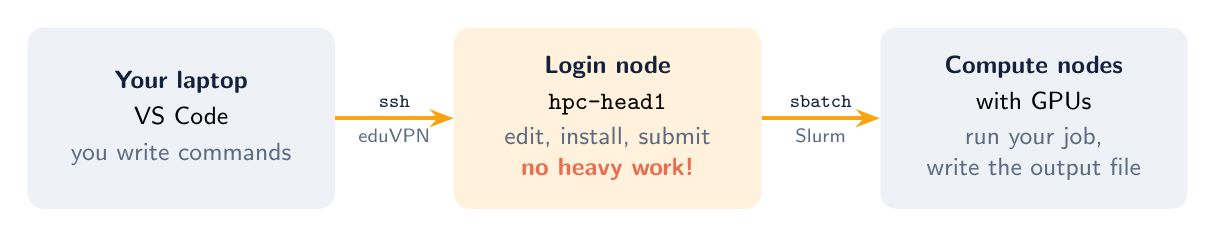
\begin{tikzpicture}[
  box/.style={draw=none, fill=tint, rounded corners=2mm, minimum width=3.9cm, minimum height=2.3cm, align=center, font=\small},
  arr/.style={-{Stealth[length=3mm]}, line width=1.4pt, amber}]
  \node[box] (lap) {\textbf{\color{navy}Your laptop}\\[0.2em]VS Code\\[0.2em]\color{slate}you write commands};
  \node[box, fill=amber!15, right=1.5cm of lap] (login) {\textbf{\color{navy}Login node}\\[0.2em]\texttt{hpc-head1}\\[0.2em]\color{slate}edit, install, submit\\\color{coral}\textbf{no heavy work!}};
  \node[box, right=1.5cm of login] (gpu) {\textbf{\color{navy}Compute nodes}\\[0.2em]with GPUs\\[0.2em]\color{slate}run your job,\\\color{slate}write the output file};
  \draw[arr] (lap) -- node[above, font=\scriptsize\ttfamily, text=navy]{ssh} node[below, font=\scriptsize, text=slate]{eduVPN} (login);
  \draw[arr] (login) -- node[above, font=\scriptsize\ttfamily, text=navy]{sbatch} node[below, font=\scriptsize, text=slate]{Slurm} (gpu);
\end{tikzpicture}
\end{center}

\begin{itemize}
  \item The \textbf{login node} is shared by everyone. Use it to edit code, install packages, and submit jobs. \textbf{Never run training or other heavy programs on it.}
  \item The \textbf{compute nodes} have the GPUs. You reach them by submitting a \textbf{job} to the scheduler, called \textbf{Slurm}.
\end{itemize}

\subsection{First connection from a terminal}
Open a terminal (Windows: \menu{PowerShell}; Ubuntu: \menu{Terminal}) and run:
\begin{cmd}
ssh s1234567@hpc-head1.ewi.utwente.nl
\end{cmd}
\begin{itemize}
  \item The first time, ssh asks \texttt{Are you sure you want to continue connecting?} Type \code{yes}.
  \item Type your UT password. \textbf{Nothing appears while you type.} This is normal. Press \key{Enter}.
\end{itemize}
If you see \texttt{Permission denied (keyboard-interactive)}, use this command instead:
\begin{cmd}
ssh -o PreferredAuthentications=password s1234567@hpc-head1.ewi.utwente.nl
\end{cmd}

\shot{b1_ssh.jpg}{The first ssh login, here from the VS Code terminal.}

\begin{checkbox}The prompt changes to something like \texttt{s1234567@hpc-head1:\textasciitilde\$}. Type \code{exit} to log out.\end{checkbox}

\subsection{Save the connection in an SSH config file}
This file lets VS Code (and you) connect with a short name.
We open the file in VS Code. (Notepad would save it as \texttt{config.txt}, which does not work.)
\begin{wincmd}
mkdir -Force $HOME\.ssh
code $HOME\.ssh\config
\end{wincmd}
\begin{ubucmd}
mkdir -p ~/.ssh
code ~/.ssh/config
\end{ubucmd}
If VS Code asks whether to open a file from outside the workspace, click \menu{Open}. Type or paste these lines, put in \textbf{your own} username, and save with \key{Ctrl+S}. VS Code indents the lines for you.
\begin{cmd}
Host ut-hpc
    HostName hpc-head1.ewi.utwente.nl
    User s1234567
    PreferredAuthentications publickey,password
\end{cmd}
\shot{b2_config.jpg}{The SSH config file in VS Code (use your own username).}

\begin{checkbox}\code{ssh ut-hpc} now logs you in. Type \code{exit} to log out.\end{checkbox}

\subsection{(Recommended) An SSH key, so you do not type your password every time}
\begin{cmd}
ssh-keygen -t ed25519
\end{cmd}
Press \key{Enter} three times (default file, no passphrase). Then copy the public key to the cluster:
\begin{wincmd}
type $HOME\.ssh\id_ed25519.pub | ssh ut-hpc "mkdir -p ~/.ssh && cat >> ~/.ssh/authorized_keys && chmod 600 ~/.ssh/authorized_keys"
\end{wincmd}
\begin{ubucmd}
ssh-copy-id ut-hpc
\end{ubucmd}
Type your password one last time.
\begin{checkbox}\code{ssh ut-hpc} logs you in \textbf{without} asking for a password.\end{checkbox}

\subsection{Connect from VS Code}
\begin{enumerate}
  \item Click the \code{><} button in the bottom-left corner of VS Code.
  \item Choose \menu{Connect to Host...} and then \menu{ut-hpc}.
  \item If asked for the platform, choose \menu{Linux}. Type your password if asked.
  \item The first connection takes about a minute: VS Code installs a small helper on the cluster.
\end{enumerate}

\shot{b4_connect.jpg}{Remote-SSH: Connect to Host, then choose ut-hpc.}

\shot{b4_connected.jpg}{Connected: the bottom-left corner shows SSH: ut-hpc.}

\begin{checkbox}The bottom-left corner shows \textbf{SSH: ut-hpc}. Open a terminal (\menu{Terminal > New Terminal}). It runs \textbf{on the cluster}: \code{hostname} prints \texttt{hpc-head1}.\end{checkbox}

\newpage
% ================= Part C =================
\section{Run a GPU job on the HPC cluster}
All commands in Part C run in the VS Code terminal that is connected to \textbf{ut-hpc}.

\subsection{Clone the project}
\begin{cmd}
mkdir -p ~/projects
cd ~/projects
git clone https://github.com/alicamdal/vscode-hpc-tutorial.git
cd vscode-hpc-tutorial
\end{cmd}
Now open the folder in VS Code: \menu{File > Open Folder...}, choose this folder and click \menu{OK} (if VS Code asks whether you trust the authors, click \menu{Yes}):\\
\texttt{/home/s1234567/projects/vscode-hpc-tutorial}
\begin{checkbox}The Explorer on the left shows the folders \texttt{demo} and \texttt{hpc}.\end{checkbox}

\subsection{Create a virtual environment}
A \textbf{virtual environment} is a private folder of Python packages for one project. Packages installed there do not change other projects or the system Python. We call the folder \texttt{.venv}.
\begin{cmd}
python3 -m venv .venv
source .venv/bin/activate
python -m pip install --upgrade pip
\end{cmd}
\begin{checkbox}The prompt now starts with \texttt{(.venv)}. \code{which python} prints a path that ends with \texttt{vscode-hpc-tutorial/.venv/bin/python}.\end{checkbox}
\begin{notebox}Each time you open a new terminal, activate the environment again with \code{source .venv/bin/activate}.\end{notebox}

\subsection{Install PyTorch}
\begin{cmd}
pip install torch numpy
\end{cmd}
This downloads about 3 GB and takes \textbf{about 3 minutes}. Wait until the prompt returns.
\begin{checkbox}\code{python -c "import torch; print(torch.\_\_version\_\_)"} prints a version such as \texttt{2.15.0+cu132}. The \texttt{cu132} part means ``built for NVIDIA GPUs (CUDA 13.2)''.\end{checkbox}

\subsection{Try the GPU check on the login node}
\begin{cmd}
python hpc/check_gpu.py
\end{cmd}
The script prints \texttt{GPU available no} and \emph{This is expected on the login node: it has no GPU.} This is the point: \textbf{the login node has no GPU.} To use one, we ask Slurm for it.

\subsection{Submit the job}
Open \texttt{hpc/check\_gpu.sbatch} in VS Code and read it. The \texttt{\#SBATCH} lines ask Slurm for resources:

\begin{tabularx}{\linewidth}{@{}l X@{}}
\toprule
\textbf{Line} & \textbf{Meaning} \\
\midrule
\texttt{--partition=students} & the group of GPU computers for courses \\
\texttt{--gres=gpu:1} & one GPU \\
\texttt{--cpus-per-task=2}, \texttt{--mem=4G} & two CPU cores and 4 GB of memory \\
\texttt{--time=00:05:00} & stop the job after at most 5 minutes \\
\texttt{--output=gpu-check-\%j.out} & write everything the job prints to this file (\texttt{\%j} = job id) \\
\bottomrule
\end{tabularx}

Submit it \textbf{from the project folder}, then watch the queue:
\begin{cmd}
sbatch hpc/check_gpu.sbatch
squeue --me
\end{cmd}
Slurm answers \texttt{Submitted batch job 123456}. In \texttt{squeue}, \texttt{PD} means waiting and \texttt{R} means running. When your job is no longer listed, it is finished. With 30 students on a few GPUs, waiting a minute or two is normal.

\subsection{Read the result}
A file \texttt{gpu-check-123456.out} appears in the Explorer. Open it, or run \code{cat gpu-check-*.out}. After the \texttt{nvidia-smi} table you see something like this (from a test run; your machine and GPU will differ):
\begin{outbox}
Where am I?
  machine                hpc-node30
  Slurm job id           733512
  partition              itc-gpu

Software
  Python                 3.12.3
  PyTorch                2.15.0+cu132
  PyTorch built for CUDA 13.2

GPU
  GPU 0                  NVIDIA RTX PRO 6000 Blackwell Server Edition
    memory (VRAM)        95.1 GB total, 94.5 GB free

Speed test: multiply two 4096 x 4096 matrices
  CPU                       996.8 ms  (  0.14 TFLOP/s)
  GPU                         1.9 ms  ( 73.31 TFLOP/s)
  GPU is faster by       532 x
\end{outbox}

\shot{c6_output.jpg}{The job output in the VS Code terminal (\texttt{cat gpu-check-*.out}).}

\begin{checkbox}The machine name is \textbf{not} \texttt{hpc-head1}. Your code ran on a compute node with a GPU.\end{checkbox}

\subsection{Rules for the cluster}
\begin{itemize}
  \item No heavy work on the login node. Always use \texttt{sbatch} (or \texttt{srun} for short interactive sessions).
  \item Ask only for what you need (\texttt{--gres}, \texttt{--mem}, \texttt{--time}). Others are waiting.
  \item Submit once, then wait. Do not submit the same job many times.
  \item The cluster is not a backup. Copy results you want to keep to your laptop.
\end{itemize}
Cluster documentation: \url{https://hpc.wiki.utwente.nl/eemcs-hpc}.
When you are done, close the remote window: \menu{File > Close Remote Connection}.

\newpage
% ================= Part D =================
\section{Run the Vision Transformer on your laptop}
Now we do the same steps (clone, environment, install, run) on your \textbf{own laptop}. The model is small (about 23 MB) and runs on a normal CPU in about a second.

\subsection{Clone the project on your laptop}
Open a \textbf{new local} VS Code window (the bottom-left corner must \textbf{not} say SSH). Open a terminal:
\begin{cmd}
cd ~/Documents
git clone https://github.com/alicamdal/vscode-hpc-tutorial.git
cd vscode-hpc-tutorial
\end{cmd}
Open the folder: \menu{File > Open Folder...} and choose \texttt{Documents/vscode-hpc-tutorial}. If VS Code asks whether you trust the authors (or shows \emph{Restricted Mode}), choose \menu{Trust}. Then open a new terminal with \menu{Terminal > New Terminal}.

\subsection{Create and activate a virtual environment}
\begin{wincmd}
py -3.13 -m venv .venv
.venv\Scripts\Activate.ps1
\end{wincmd}
If PowerShell says \emph{running scripts is disabled on this system}, run this once and try again:
\begin{wincmd}
Set-ExecutionPolicy -Scope CurrentUser RemoteSigned
\end{wincmd}
\begin{ubucmd}
python3 -m venv .venv
source .venv/bin/activate
\end{ubucmd}
Then, on both systems:
\begin{cmd}
python -m pip install --upgrade pip
\end{cmd}
Tell VS Code to use this environment too: press \key{Ctrl+Shift+P}, type \menu{Python: Select Interpreter}, and choose the entry with \texttt{.venv}.

\shot{d2_interpreter.jpg}{Python: Select Interpreter, then the .venv entry.}

\begin{checkbox}The prompt starts with \texttt{(.venv)}.\end{checkbox}

\subsection{Install packages one by one}
First PyTorch. We install the CPU version of PyTorch. It is a much smaller download, so the installation is quick, and our small model runs fast on a CPU. Because it goes into the virtual environment, the Python installation of your laptop does not change.
\begin{wincmd}
pip install torch
\end{wincmd}
\begin{ubucmd}
pip install torch --index-url https://download.pytorch.org/whl/cpu
\end{ubucmd}
On Windows, pip installs the CPU version by default. On Ubuntu, without the extra address pip downloads the much larger GPU version. Then the Hugging Face library that downloads and runs the model:
\begin{cmd}
pip install transformers
\end{cmd}
\begin{checkbox}\code{pip list} shows \texttt{torch} and \texttt{transformers}.\end{checkbox}

\subsection{Install the rest from requirements.txt}
Installing packages one by one is fine for two packages. Real projects need many, with known versions. They are listed in a file called \texttt{requirements.txt}. Open it in VS Code and look at it.
\begin{cmd}
pip install -r requirements.txt
\end{cmd}
pip says \texttt{Requirement already satisfied} for the packages you already have and installs the rest (for example \texttt{matplotlib}).
\begin{notebox}[Why did we install torch first?]
On Ubuntu, \code{pip install -r requirements.txt} alone would pick the large GPU version of torch. Installing the CPU version first keeps the download small.
\end{notebox}

\subsection{Run the demo}
\begin{cmd}
python demo/vit_demo.py
\end{cmd}
The first run downloads the model (about 23 MB). The program prints each step:
\begin{outbox}
[Step 4] Cut the image into patches
  224 / 16 = 14 patches per side, 14 x 14 = 196 patches
  each patch has 16 x 16 x 3 = 768 pixel values

[Step 5] Run the transformer
  tokens per image: 197 = 1 class token + 196 patch tokens
  each token is a vector of 192 numbers (the embedding)
...
[Step 7] Prediction
   11.0 %  Egyptian cat
    7.8 %  tabby
    6.6 %  tiger cat
\end{outbox}
\shot{d5_demo_run.jpg}{The demo finished on Windows. The figures are in outputs/cat.}

\begin{checkbox}The folder \texttt{outputs/cat/} contains five images. Click them in the VS Code Explorer.\end{checkbox}

\subsection{What the five figures show}

\begin{center}
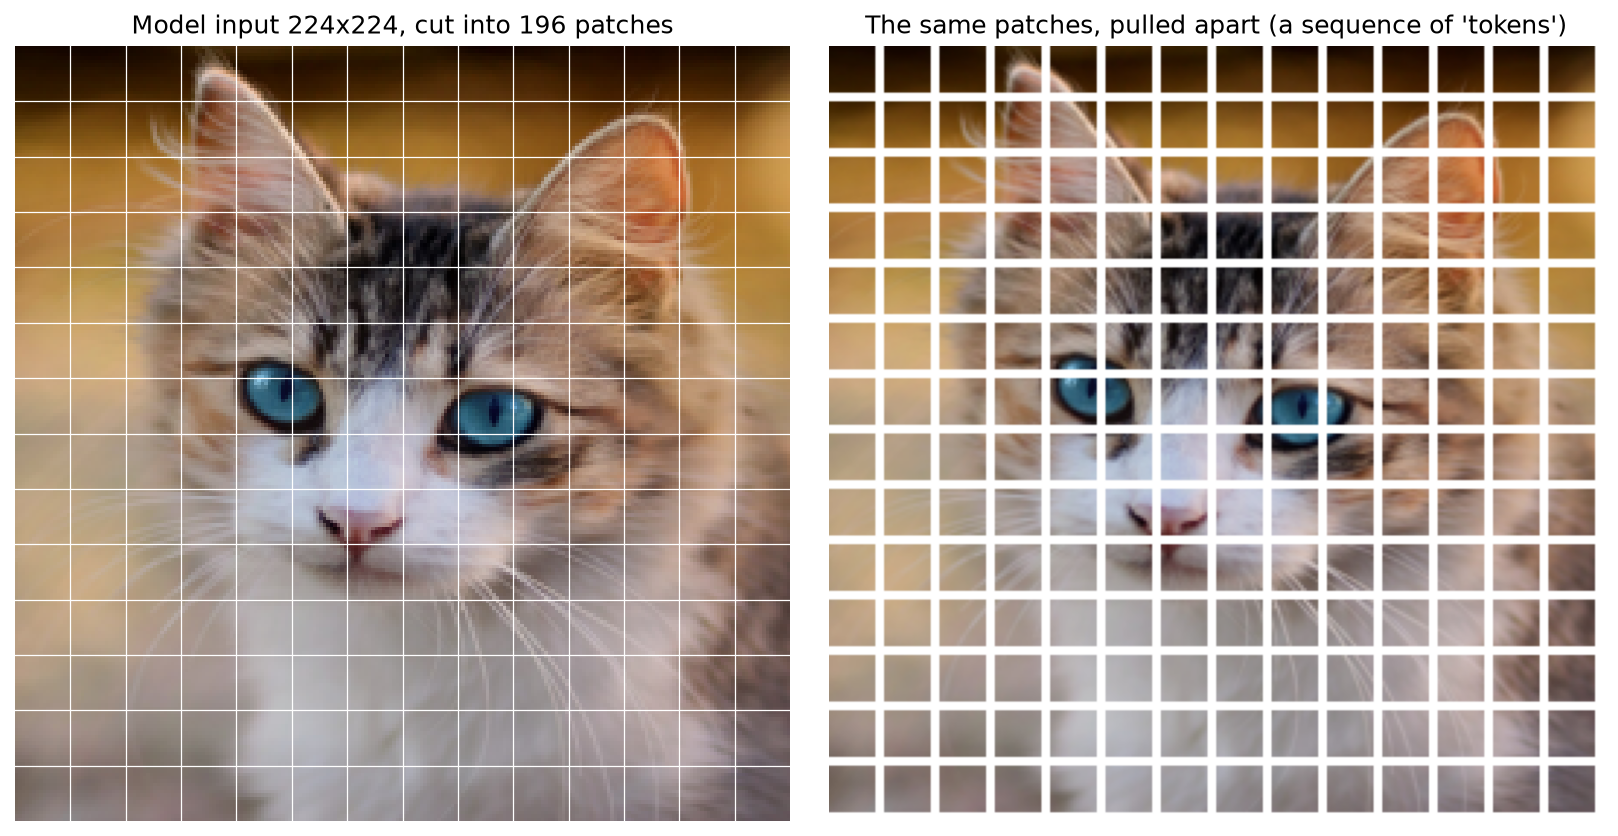
\includegraphics[width=0.92\linewidth]{img/demo_1_patches.png}\\
{\small\color{slate}\textbf{1\_patches.png} The 224\,$\times$\,224 input cut into a 14\,$\times$\,14 grid. A transformer reads the image as a \textbf{sequence} of 196 patches, like words in a sentence.}
\end{center}

\begin{center}
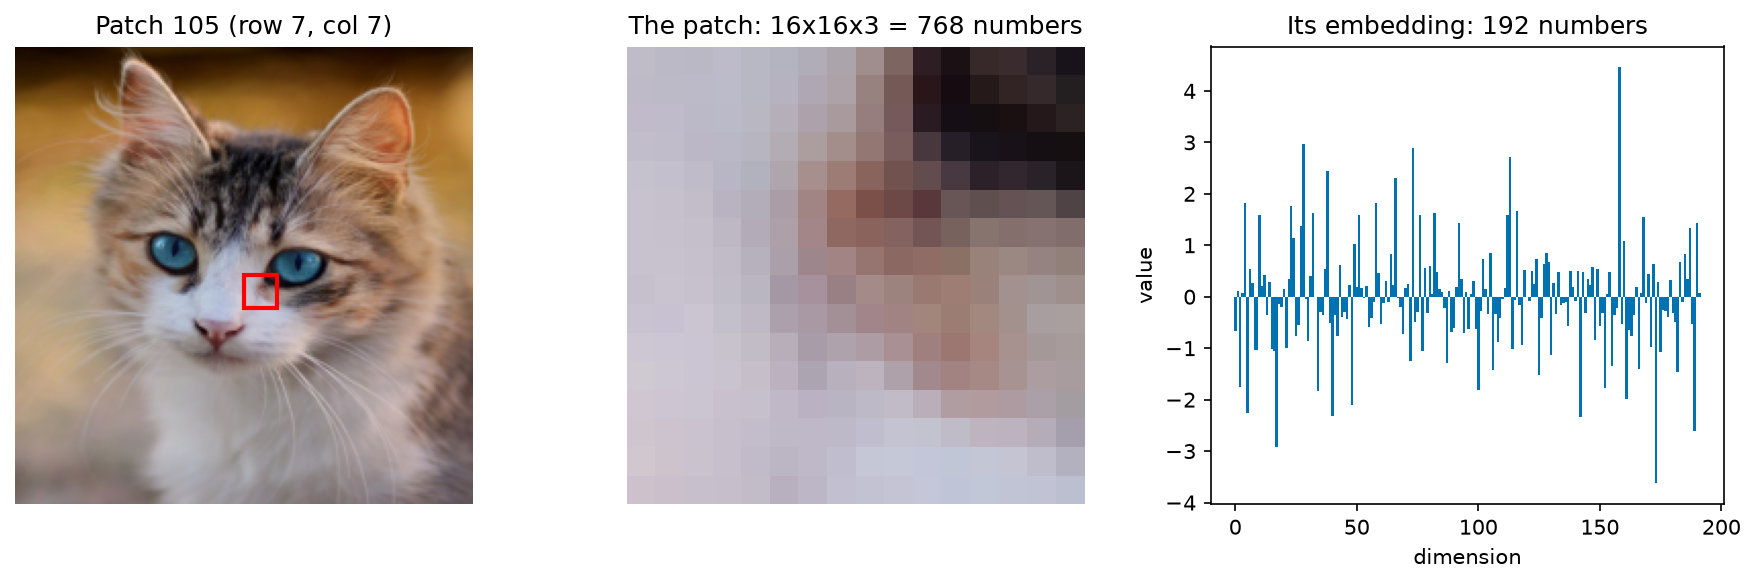
\includegraphics[width=0.92\linewidth]{img/demo_2_patch_embedding.png}\\
{\small\color{slate}\textbf{2\_patch\_embedding.png} One patch (768 pixel values) becomes a vector of 192 numbers: its \textbf{embedding}.}
\end{center}

\begin{center}
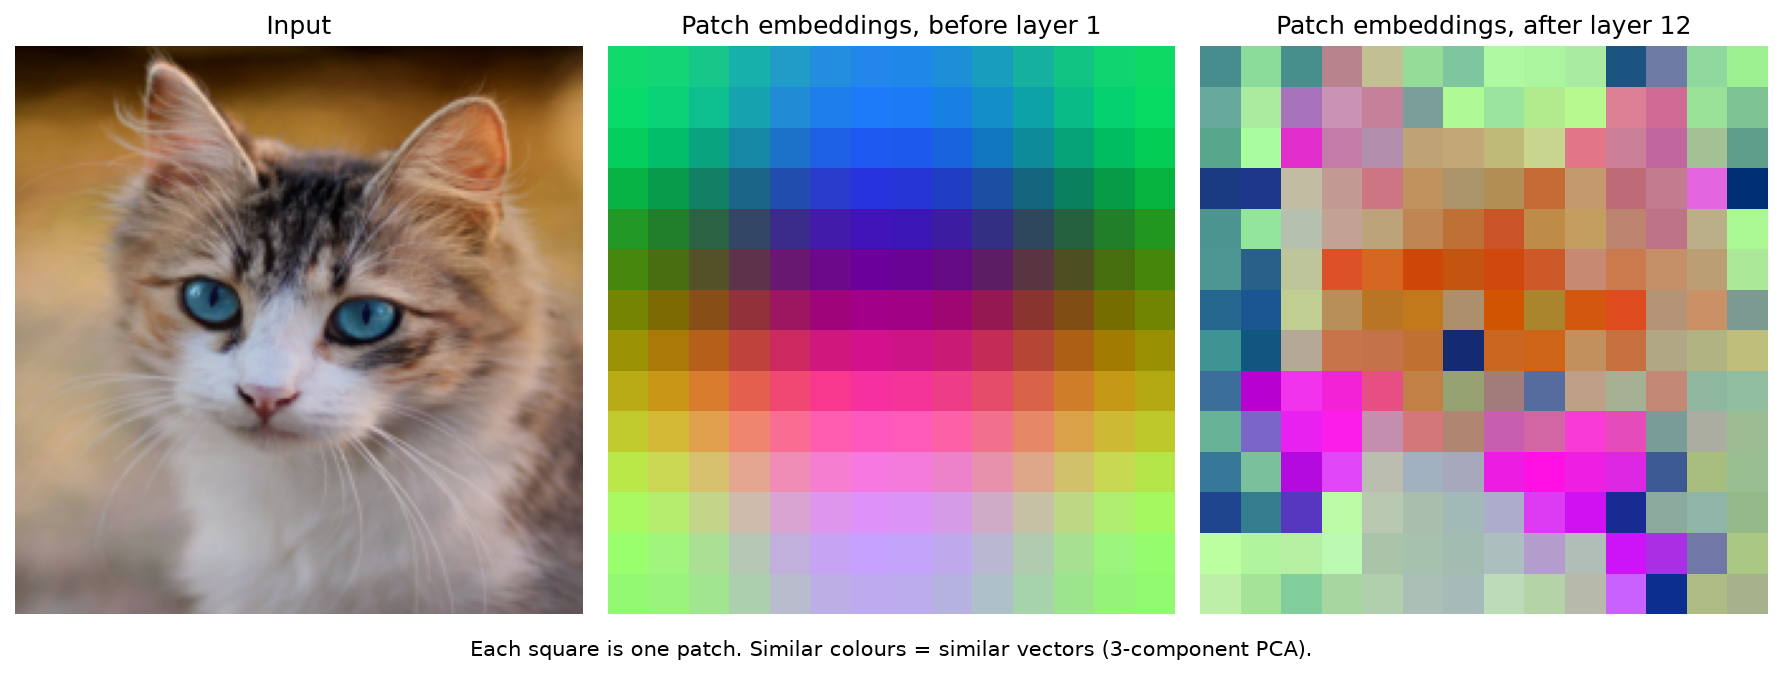
\includegraphics[width=0.92\linewidth]{img/demo_3_embeddings_pca.png}\\
{\small\color{slate}\textbf{3\_embeddings\_pca.png} All patch vectors shown as colours. Before layer 1 the colours mostly show \textbf{position}. After 12 layers they show \textbf{content}: cat and background separate.}
\end{center}

\begin{center}
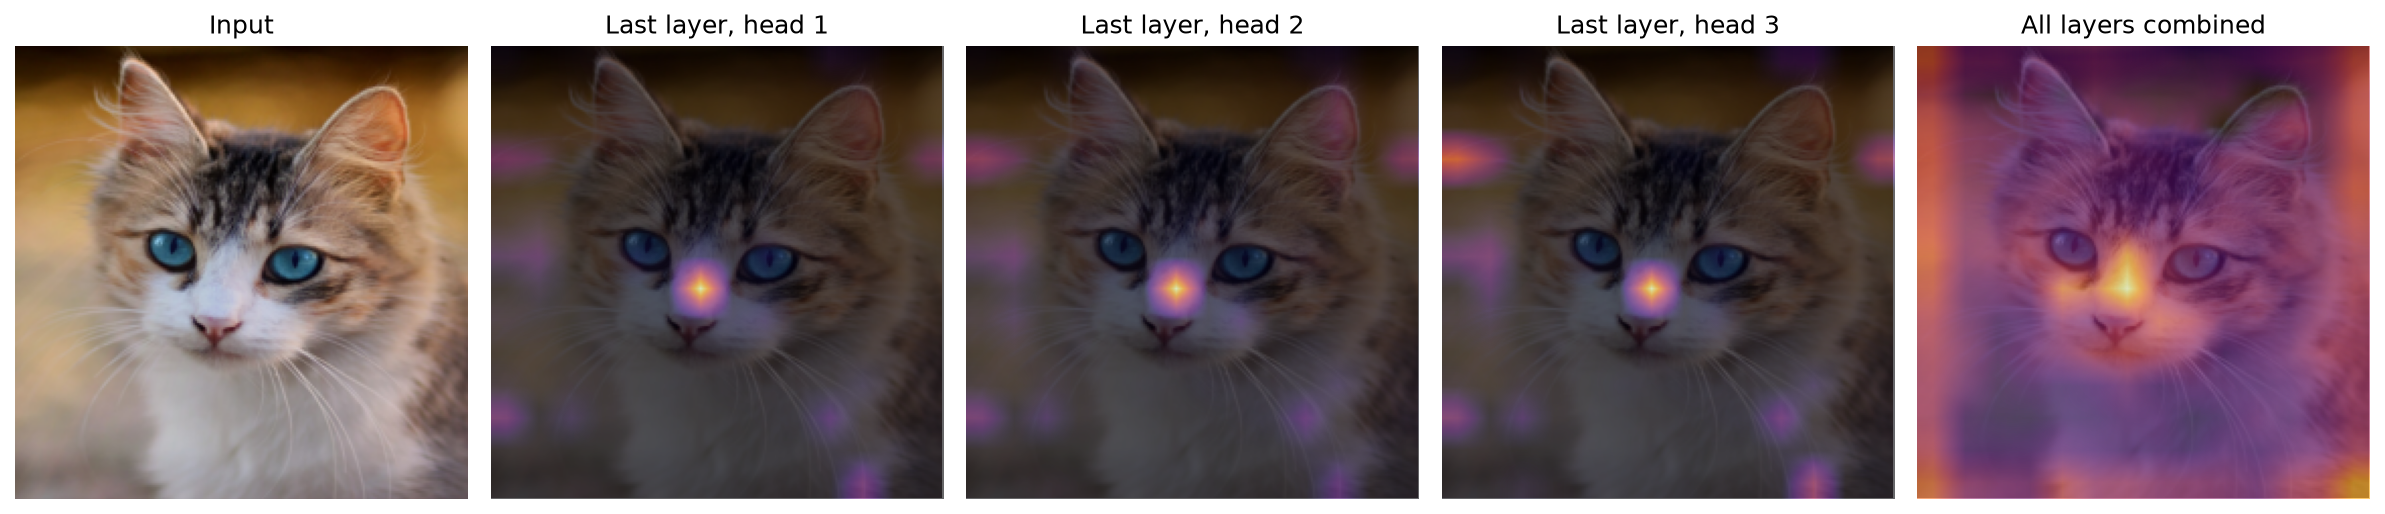
\includegraphics[width=0.92\linewidth]{img/demo_4_attention.png}\\
{\small\color{slate}\textbf{4\_attention.png} Where the class token looks, for each of the 3 heads of the last layer and over all layers combined. Attention is how tokens share information.}
\end{center}

\begin{center}
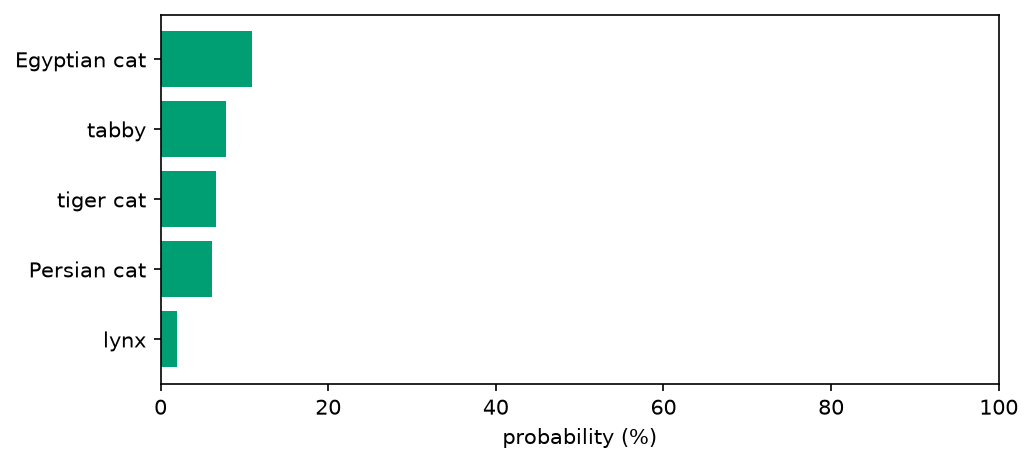
\includegraphics[width=0.6\linewidth]{img/demo_5_prediction.png}\\
{\small\color{slate}\textbf{5\_prediction.png} The five most likely of the 1000 ImageNet classes.}
\end{center}

\subsection{Try it yourself}
\begin{cmd}
python demo/vit_demo.py --image demo/images/fox.jpg
python demo/vit_demo.py --image demo/images/bus.jpg
python demo/vit_demo.py --image demo/images/cat.jpg --patch 0
\end{cmd}
\begin{itemize}
  \item The fox picture is a 19th-century \textbf{painting}, not a photo. Is the prediction still right?
  \item Take a photo with your phone and run the script on it. Which objects work well, and which do not?
  \item Look at \code{--patch 0} (top-left corner). How does its embedding differ from a patch on the cat?
\end{itemize}

\newpage
% ================= Part E =================
\section{(Optional) An AI coding assistant}
\textbf{GitHub Copilot} suggests code and answers questions about your code inside VS Code.
\begin{itemize}
  \item Everyone with a GitHub account can use the limited \textbf{Copilot Free} plan.
  \item Verified students can get the \textbf{Copilot Student} plan for free through GitHub Education (\url{https://github.com/education}). Verification can take a few days.
\end{itemize}
To start:
\begin{enumerate}
  \item In VS Code, click the \menu{Copilot} icon in the top bar (or the Accounts icon, bottom left) and \textbf{sign in with GitHub}.
  \item Open the \menu{Chat} view (\key{Ctrl+Alt+I}).
  \item Open \texttt{demo/vit\_demo.py} and try:
  \begin{itemize}
    \item \emph{``Explain what the function attention\_rollout does, in simple words.''}
    \item \emph{``Add a --top option that sets how many predictions are printed.''}
  \end{itemize}
\end{enumerate}

\begin{notebox}[Important]Always read and test what the assistant writes. It can be wrong. Follow the course rules on using AI tools.\end{notebox}

% ================= Troubleshooting =================
\section*{Troubleshooting}\label{sec:trouble}
\renewcommand{\arraystretch}{1.3}
\begin{tabularx}{\linewidth}{@{}>{\raggedright\arraybackslash}p{0.38\linewidth} X@{}}
\toprule
\textbf{Problem} & \textbf{Solution} \\
\midrule
\texttt{ssh: connect to host ... Connection timed out} & You are not on the UT network. Connect eduVPN (Institute Access, University of Twente). \\
\texttt{Permission denied (keyboard-interactive)} & Add\newline \texttt{-o PreferredAuthentications=password}\newline (B1), or check the config file (B2). \\
\texttt{Permission denied (password)} & Wrong username or password. The username is lowercase, for example \texttt{s1234567}. \\
The ssh config was saved as \texttt{config.txt} & Rename it in PowerShell:\newline \texttt{Rename-Item \$HOME\textbackslash.ssh\textbackslash config.txt config} \\
VS Code hangs on ``Setting up SSH host'' & Close the window and connect again. If it keeps failing: \key{Ctrl+Shift+P}, \menu{Remote-SSH: Kill VS Code Server on Host}. \\
\texttt{sbatch: error: invalid partition} or \texttt{Invalid account} & Your account is not yet enabled for the \texttt{students} partition. Tell the TA. \\
The job stays \texttt{PD} for a long time & Other jobs use the GPUs. Wait; do not submit the job many times. \\
\texttt{py} or \texttt{git} not found (Windows) & Close and reopen VS Code. If it still fails, re-run the Python installer, choose \menu{Modify}, and tick \menu{Add Python to environment variables}. \\
\texttt{python3 -m venv} fails (Ubuntu) & \texttt{sudo apt install python3-venv} \\
Ubuntu 22.04: Python is 3.10, torch will not install & Install Python 3.11 or newer, or upgrade to Ubuntu 24.04. Ask the TA. \\
\texttt{pip install torch} is very slow or huge on Ubuntu & You forgot the CPU address (D3):\newline \texttt{--index-url}\newline \url{https://download.pytorch.org/whl/cpu} \\
\texttt{OSError: [WinError 126]} \texttt{... c10.dll} (Windows) & Install the Microsoft Visual C++ Redistributable (A5), then run the script again. \\
\texttt{No module named 'torch'} & The environment is not active. Run the activate command (D2) and look for \texttt{(.venv)}. \\
The model download fails & Check your internet connection and run the script again. \\
\bottomrule
\end{tabularx}

\end{document}
